\section{Množiny a čísla}\label{sec:mnoziny_a_cisla}

V této sekci si připomeneme některá značení pro práci s čísly, zavedeme nová a především připomeneme práci s množinami.

\subsection{Čísla a sumy}

\begin{convention}[Značení číselných oborů]
    V dalším textu budeme obor \emph{přirozených čísel} značit písmenem $\N$, obor \emph{celých čísel} písmenem $\Z$, obor \emph{racionálních čísel} písmenem $\Q$, obor \emph{reálných čísel} písmenem $\R$ a obor komplexních čísel písmenem $\C$. Speciálně, horním indexem "$+$", resp. "$-$", budeme značit, že uvažujeme pouze všechna kladná, resp. záporná, čísla a dolním indexem "$0$" budeme značit, že v~dané množině uvažujeme nulu. (Např. $\R_0^+$, $\N_0$, $\Z^-$, apod.) 
\end{convention}

Číselné intervaly budeme zapisovat pomocí kulatých závorek $(,)$ pro otevřené nebo polootevřené intervaly a pro uzavřené nebo polouzavřené intervaly budeme používat\footnote{V jiných textech se mohou používat i hranaté závorky $[,]$.} špičaté závorky $\langle,\rangle$.\par
\medskip
Při sčítání většího počtu čísel pro nás bude výhodnější zavést značení pomocí symbolu $\sum$ (velké řecké písmeno "sigma")\footnote{Pokud se čtenář někdy setkal s programováním (v libovolném jazyce), tento zápis svým způsobem připomíná \texttt{FOR} cyklus.}. Mějme nějakou číselnou posloupnost $a_1,a_2,\dots,a_n$. Pak součet $a_1+a_2+\cdots+a_n$ můžeme zapsat ve tvaru
\begin{equation*}
    \sum_{i=1}^{n}{a_i}.
\end{equation*}
\begin{example}\label{ex:uziti_sum}
    Příklady různých součtů zapsaných pomocí sumy:
    \begin{enumerate}[label=(\roman*)]
        \item $\displaystyle \sum_{i=1}^{5}{i}=1+2+3+4+5$ ,
        \item $\displaystyle \sum_{i=1}^{10}{\dfrac{1}{3i}}=\dfrac{1}{3}+\dfrac{1}{6}+\dfrac{1}{9}+\cdots+\dfrac{1}{27}+\dfrac{1}{30}$ ,
        \item $\displaystyle \sum_{j=1}^{5}{\dfrac{1}{3i}}=\dfrac{1}{3i}+\dfrac{1}{3i}+\dfrac{1}{3i}+\dfrac{1}{3i}+\dfrac{1}{3i}=\dfrac{5}{3i}$ .
    \end{enumerate}
\end{example}
Symbol sumy se může i kumulovat pro zápis složitějších součtů:
\begin{align*}
    \sum_{i=1}^{n}{\sum_{j=1}^{m}{(i+j)}}&=\sum_{i=1}^{n}{\left((i+1)+(i+2)+\cdots+(i+m)\right)}=\\
    &=(1+1)+(1+2)+\cdots+(1+m)+\\
    &+(2+1)+(2+2)+\cdots+(2+m)+\\
    &+(3+1)+(3+2)+\cdots+(3+m)+\\
    &\vdots\\
    &+(n+1)+(n+2)+\cdots+(n+m).
\end{align*}
V některých textech se u dvojité sumy připisují závorky k~vnitřní sumě
\begin{equation*}
    \sum_{i=1}^{n}{\left(\sum_{j=1}^{m}{(i+j)}\right)}.
\end{equation*}
My se však budeme držet varianty bez závorek (nebude-li potřeba je použít).\par
Podobně můžeme zapisovat i součiny čísel (tzv. \emph{produkt}) pomocí symbolu $\prod$ (velké řecké písmeno "pí"):
\begin{equation*}
    \prod_{i=2}^{n}{\dfrac{i+1}{i-1}}=\dfrac{3}{1}\cdot\dfrac{4}{2}\cdot\dfrac{5}{3}\cdots\dfrac{n-1}{n-3}\cdot\dfrac{n}{n-2}\cdot\dfrac{n+1}{n-1}=\dfrac{n(n+1)}{2}.
\end{equation*}

\subsection{Množiny a operace s nimi}\label{subsec:mnoziny_a_operace_s_nimi}

Množinami se budeme v~tomto textu ještě podrobněji zabývat; nyní si však pouze připomeneme, co už víme. Množiny zapisujeme pomocí složených závorek $\{,\,\}$ a pro jejich označování si vymezíme velká písmena latinské abecedy\linebreak $A,\,B,\,C,\,D,\dots,\,X,\,Y,\,Z$, kterou případně opět opatříme indexy. Např. množinu s prvky 10, 4, 90, 666 zapíšeme jako $\set{4, 10, 90, 666}$. Speciálně, prázdnou množinu značíme buď $\emptyset$ nebo $\{\}$. Prvky v~množině budeme vždy seřazovat vzestupně, pokud nebude v~dané situaci výhodnější použít jiné uspořádání.\par
Kromě zápisu množin samotných bude často potřeba vyjádřit, že nějaká množina obsahuje jistý prvek. K tomu používáme symbol "$\in$". Tedy např. informaci, že množina $X$ obsahuje prvek $x$ píšeme jako $x\in X$ (čteme "$x$ je prvkem (množiny) $X$"). Opačný případ, kdy prvek $x$ nenáleží množině $X$ budeme zapisovat jako $x \notin X$. (Jedná se v~podstatě o zkrácený zápis formule $\neg (x \in X)$.)\par
Mějme množiny
\begin{equation*}
    A=\set{333, 444, 555}\quad\text{a}\quad B=\set{333, 333, 444, 444, 555}.
\end{equation*}
Jsou množiny $A$ a $B$ odlišné? \textbf{Ne, nejsou}; u množin neuvažujeme násobné výskyty prvků, ale pouze, zdali mají či nemají stejné prvky. Tj. množiny $X$ a $Y$ považujeme za rovné, což vyjadřujeme pomocí "=", tedy $X=Y$ (formálně zavedeme v~sekci \todo{Doplnit sekci na axiomy TM}), v opačném případě píšeme $X \neq Y$.\par
Řadu množin v~matematice definujeme pomocí jiných množin na základě jistého pravidla. Např. množinu všech mocnin dvojky bychom zapsali jako
\begin{equation*}
    \set{2^n \admid n \in \N}=\set{2^1, 2^2, 2^3, \dots}.
\end{equation*}

\begin{example} Další zápisy množin podle společné vlastnosti prvků:
    \begin{enumerate}[label=(\roman*)]
        \item $\set{2k-1 \admid k \in \N}=\set{k\in\N \admid k\;\text{je liché}}=\set{1,\,3,\,5,\,7,\,\dots}$ ,
        \item $\set{i^2 \admid i \in \N}=\set{n \in \N \admid \exists k\in\N: k^2=n}=\set{1,\,4,\,9,\,16,\,\dots}$
        \item 
        \begin{align*}
            \set{\sqrt{n} \admid n \in \N}&=\set{x \in \R \admid x \geq 1 \land \exists n\in\N: x^2=n}=\\
            &=\set{\sqrt{1},\,\sqrt{2},\,\sqrt{3},\,\sqrt{4},\,\dots}.
        \end{align*}
    \end{enumerate}
\end{example}
\begin{remark}
    V případě slovního popisu společné vlastnosti je třeba dbát na jednoznačnost.
\end{remark}

U množin můžeme jako jejich prvky vzít i jiné množiny, např.:
\begin{equation}\label{eq:system_mnozin}
    M_1=\set{\set{1,2,3},\set{\set{8,14},3},\set{0,7}, \set{3}, \set{5}},
\end{equation}
přičemž i takové typy množiny můžeme zadat společnou vlastností:
\begin{equation*}
    M_2=\set{\set{i,j,k} \admid i,j,k\in\N}.
\end{equation*}
Abychom nemuseli říkat "množina množin", používáme název \emph{systém množin} nebo též \emph{množinový systém}.
\begin{convention}
    Pro systémy množin budeme používat velké kaligrafické písmo latinské abecedy $\mathcal{A},\mathcal{B},\mathcal{C},\mathcal{D},\dots,\mathcal{X},\mathcal{Y},\mathcal{Z}$.
\end{convention}
U množin nás dále bude zajímat jejich \emph{mohutnost}, kterou budeme značit svislými čarami, tj. $\sizeof{X}$. Později si tento termín zavedeme i pro nekonečné množiny. Např. mohutnost množiny $X=\set{2,3,5,8}$ je $\sizeof{X}=4$. Nyní otázka na čtenáře, jakou mohutnost má množina $M_1$ uvedená v \eqref{eq:system_mnozin}? Zde je velmi důležité si uvědomit, co je prvkem množiny $M_1$. Např. číslo 1 není prvkem $M_1$, ačkoliv je prvkem množiny $\set{1,2,3}$. Prvky $M_1$ jsou pouze samotné množiny, tedy $\sizeof{M_1}=5$.\par
\medskip
Nyní zavedeme dva důležité pojmy, a to sice \emph{podmnožina} a \emph{vlastní podmnožina}. Ačkoliv tyto termíny čtenář možná již zná, přesto je pro nás poměrně důležité stanovit si jejich význam a značení k nim, neboť s nimi dále budeme pracovat.
\begin{definition}[Podmnožina a vlastní podmnožina]\label{def:podmnozina}
    Nechť $A$ a $B$ jsou množiny. Pokud platí
    \begin{equation*}
        \forall x\in B: x\in A,
    \end{equation*}
    pak říkáme, že $B$ je \emph{podmnožinou} $A$, což zapisujeme jako $B \subseteq A$. Speciálně, pokud navíc platí, že $A \neq B$, pak říkáme, že $B$ je \emph{vlastní podmnožinou} $A$ a píšeme $B \subset A$.
\end{definition}
Méně formálně řečeno, množina $B$ je podmnožinou $A$, pokud každý prvek v $B$ je obsažen i v $A$. Není zcela těžké vidět, že je-li množina $B$ vlastní podmnožinou $A$, tj. $B \subset A$, pak je i $B \subseteq A$, ovšem opačné tvrzení (obecně) neplatí.
\begin{remark}
    Vztah "$\subseteq$" se nazývá \emph{inkluze}.
\end{remark}
\begin{example}
    Příklady vztahů množin $A,\,B$ mezi sebou:
    \begin{enumerate}[label=(\roman*)]
        \item $M_1=\set{1,2},\; M_2=\set{1,2,3}$, pak platí $M_1 \subset M_2$ a tj. i $M_1 \subseteq M_2$, ale nikoliv $M_2 \subseteq M_1$ ;
        \item $N_1=\set{a,b,c},\; N_2=\set{a,b,c}$, pak platí $N_1 \subseteq N_2$ a i $N_2 \subseteq N_1$, ale nikoliv $N_1 \subset N_2$ nebo $N_2 \subset N_1$ ;
        \item $K_1=\emptyset,\; K_2=\set{k}$, pak platí $K_1 \subset K_2$ a tudíž i $K_1 \subseteq K_2$.
    \end{enumerate}
\end{example}
Zde se hodí ještě upozornit na to, že prázdná množina je podmnožinou \textbf{každé množiny}. Dalším důležitým termínem pro nás bude \emph{potenční množina}, neboli \textbf{množina všech podmnožin} dané množiny.
\begin{definition}[Potenční množina]\label{def:potence}
    Nechť $X$ je libovolná množina. \emph{Potenční množinou} (též jen \emph{potencí}) množiny $X$ nazveme množinu $\powset{X}$, když platí
    \begin{equation*}
        \forall A \left(A \in \powset{X} \iff A \subseteq X\right).
    \end{equation*}
    (značení $\mathcal{P}$ vychází z anglického "power set")\footnote{Též se občas využívá značení $2^{X}$.}
\end{definition} 
\begin{example}\label{ex:potence}
    Příklady potenčních množin:
    \begin{enumerate}[label=(\roman*)]
        \item $\powset{\set{a,b}}=\set{\emptyset,\set{a},\set{b},\set{a,b}}$ ,
        \item $\powset{\set{1,2,3}}=\set{\emptyset,\set{1},\set{2},\set{3},\set{1,2},\set{1,3},\set{2,3},\set{1,2,3}}$ ,
        \item $\powset{\emptyset}=\set{\emptyset}$ (potence má jeden prvek).
    \end{enumerate}
\end{example}
Pozorný čtenář si možná všiml, že počet podmnožin množin z příkladu \ref{ex:potence} je vždy mocninou dvojky. Skutečně, pro každou konečnou $n$-prvkovou množinu platí, že $\sizeof{\powset{X}}=2^n$, což si později i dokážeme.
Přesuňme se k~množinovým operacím. Čtenář nejspíše již zná operace \emph{sjednocení}, \emph{průniku} a \emph{rozdílu} dvou množin. Sjednocením množin $A$ a $B$ jsme rozuměli množinu, která obsahovala prvky ležící v $A$ nebo v $B$, průnikem množinu prvků ležících v $A$ i v $B$ a rozdílem množinu prvků ležících v $A$, ale nikoliv v $B$. Zadefinujme si tyto operace trochu formálněji v \ref{def:zakladni_mnozinove_operace}. 
\begin{definition}[Základní množinové operace]\label{def:zakladni_mnozinove_operace}
    Mějme množiny $A$ a $B$. Pak definujeme:
    \begin{enumerate}[label=(\roman*)]
        \item \emph{sjednocení} $A \cup B=\set{x \admid x \in A \lor x \in B}$ ,
        \item \emph{průnik} $A \cap B=\set{x \admid x \in A \land x \in B}$ ,
        \item \emph{rozdíl} $A \setminus B=\set{x \admid x \in A \land x \notin B}$ .
    \end{enumerate}
\end{definition}

Podobně jako u sumy $\sum$ a produktu $\prod$, i zde můžeme sjednocení a průnik zapsat pomocí velkých operátorů $\bigcup$ a $\bigcap$. Tj. máme-li množiny $X_1,\,\dots,\,X_n$, pak jejich sjednocení můžeme zapsat jako
\begin{equation*}
    \bigcup\limits_{i=1}^{n}{X_i}=X_1 \cup X_2 \cup \cdots \cup X_n\;
\end{equation*}
a průnik jako
\begin{equation*}
    \bigcap\limits_{i=1}^{n}{X_i}=X_1 \cap X_2 \cap \cdots \cap X_n.
\end{equation*}
Pro obě operace platí jak \emph{komutativní}, tak i \emph{asociativní zákon}:
\begin{align*}
    X \cup Y&=Y \cup X,\\
    X \cap Y&=Y \cap X,\\
    (X \cup Y) \cup Z &= X \cup (Y \cup Z),\\
    (X \cap Y) \cap Z &= X \cap (Y \cap Z).
\end{align*}
Navíc sjednocení a průnik jsou vzájemně vůči sobě \emph{distributivní}:
\begin{align*}
    X \cup (Y \cap Z) &= (X \cup Y) \cap (X \cup Z),\\
    X \cap (Y \cup Z) &= (X \cap Y) \cup (X \cap Z).
\end{align*}
Tento poznatek můžeme zobecnit užitím velkých operátorů $\bigcup,\;\bigcap$ jako
\begin{align*}
    A \cup \left(\bigcap\limits_{i=1}^{n}{X_i}\right)&=\bigcap\limits_{i=1}^{n}{(A \cup X_i)},\\
    A \cap \left(\bigcup\limits_{i=1}^{n}{X_i}\right)&=\bigcup\limits_{i=1}^{n}{(A \cap X_i)}.
\end{align*}

Ještě jedny známé vztahy pro množiny jsou tzv. \emph{de Morganovy vzorce}
\begin{align*}
    A \setminus \left(\bigcup\limits_{i=1}^{n}{X_i}\right)&=\bigcup\limits_{i=1}^{n}{(A \setminus X_i)}\\
    A \setminus \left(\bigcap\limits_{i=1}^{n}{X_i}\right)&=\bigcap\limits_{i=1}^{n}{(A \setminus X_i)}
\end{align*}
Později si ukážeme i jejich důkaz (viz sekce \ref{sec:dukaz_neprimy}). Platnost de Morganových vzorců lze i pěkně graficky znázornit pomocí Vennových diagramů (viz obrázek \ref{fig:vennuv_diagram_de_morgan}}).
\begin{figure}[H]
	\centering
	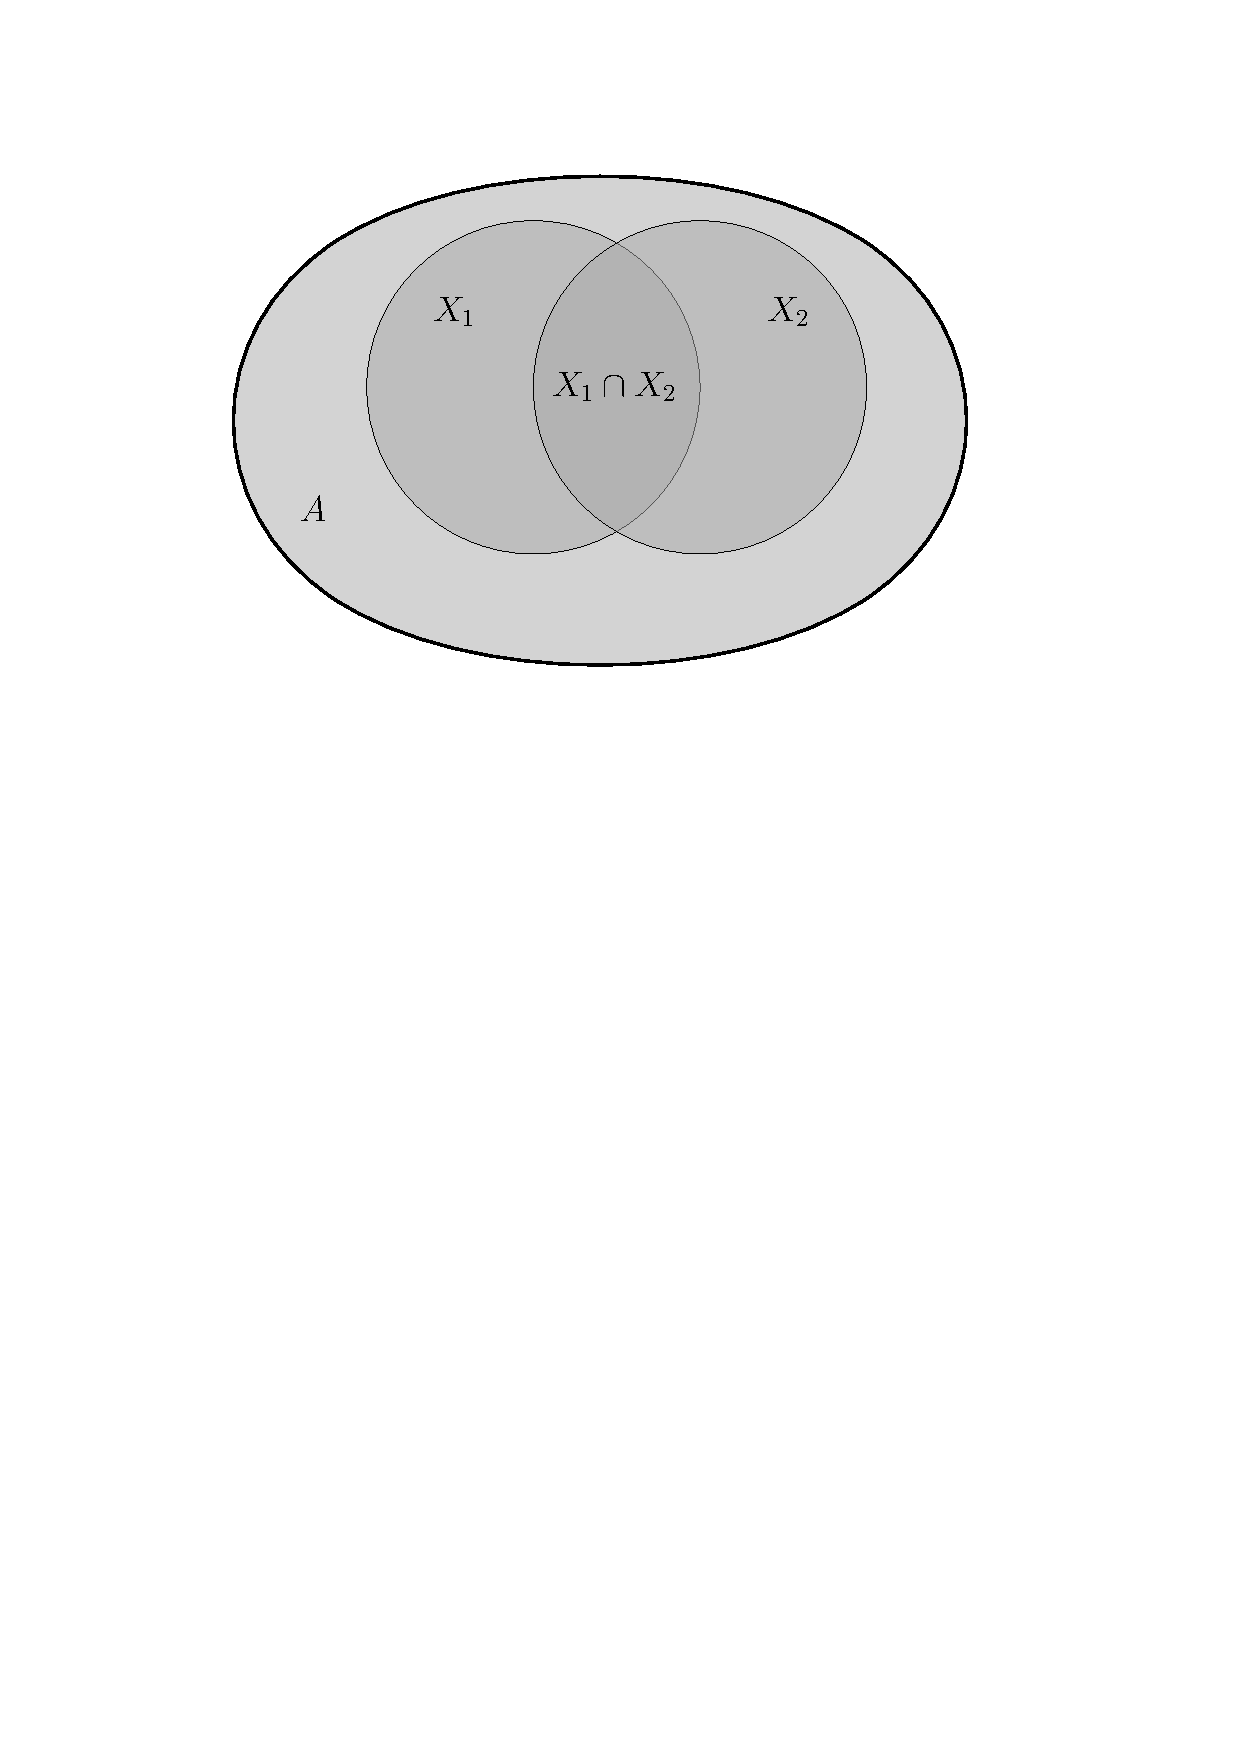
\includegraphics[scale=\normalipe]{ch02_de_Morganovy_vzorce.pdf}
    \caption{Vennův diagram pro de Morganovy vzorce při $n=2$.}
    \label{fig:vennuv_diagram_de_morgan}
\end{figure}

\begin{definition}[Disjunktní množiny]
    Nechť $\mathcal{M}$ je množinový systém. Pokud
    \begin{equation*}
        \forall X,Y\mathcal{M},\;X\neq Y: X \cap Y=\emptyset,
    \end{equation*}
    pak říkáme, že množiny $X\in\mathcal{M}$ jsou (navzájem) \emph{disjunktní}.
\end{definition}
Slovně můžeme říci, že množiny $X$ a $Y$ jsou \emph{disjunktní}, mají-li prázdný průnik.
\begin{example}
    $ $
    \begin{enumerate}[label=(\roman*)]
        \item Množiny $\set{1,2,3}$ a $\set{4,5,6}$ jsou disjunktní.
        \item Množiny $\set{1}$, $\set{2}$, $\set{1,2,3}$ nejsou disjunktní, protože $\set{1}\cap\set{1,2,3}=\set{1}$ a $\set{2}\cap\set{1,2,3}=\set{2}$.
        \item Množiny $\Q$ a $\R\setminus\Q$ (iracionální čísla) jsou disjunktní.
        \item Množiny $\R$ a $\C$ nejsou disjunktní, protože $\R\cap\C=\R$.
    \end{enumerate}
\end{example}

\subsection{Ještě k velkým operátorům}\label{subsec:dodatek_velke_operatory}

Po připomenutí práce s množinami se hodí ještě zmínit jiné způsoby zápisů pomocí velkých operátorů. Množinu, přes kterou sčítáme nemusíme nutně zadávat pouze počátečním a koncovým indexem, ale můžeme ji zadat i explicitně. Tedy např. sumu
\begin{equation*}
    \sum_{i=1}^{4}{i}
\end{equation*}
lze zapsat i třeba takto:
\begin{equation*}
    \sum_{i \in \set{1,2,3,4}}{i}=1+2+3+4.
\end{equation*}
Obecněji řečeno, pod znaménko sumy zapíšeme sčítací proměnnou a poté specifikujeme množinu hodnot, přes kterou sčítáme. Třeba součet $2^2+3^2+4^2+5^2$ můžeme zapsat jako
\begin{equation*}
    \sum_{2 \leq i \leq 5}{i^2}.
\end{equation*}
Zápis může být (stejně jako u množin) částečně nebo úplně zadán slovně. Třeba:
\begin{equation*}
    \sum_{\substack{0 \leq i \leq n\\ i\;\text{sudé}}}{i}-\sum_{\substack{0 \leq j \leq n\\ j\;\text{liché}}}{j}.
\end{equation*}
Podobně můžeme tyto způsoby zápisů využít i u jiných velkých operátorů. (Inspirováno \cite{MatousekNesetril2009}.)